\documentclass{standalone}
\usepackage{tikz}
\usetikzlibrary{patterns, positioning}
\usepackage[sfdefault]{ClearSans} %% option 'sfdefault' activates Clear Sans as the default text font
\usepackage[T1]{fontenc}

\begin{document}
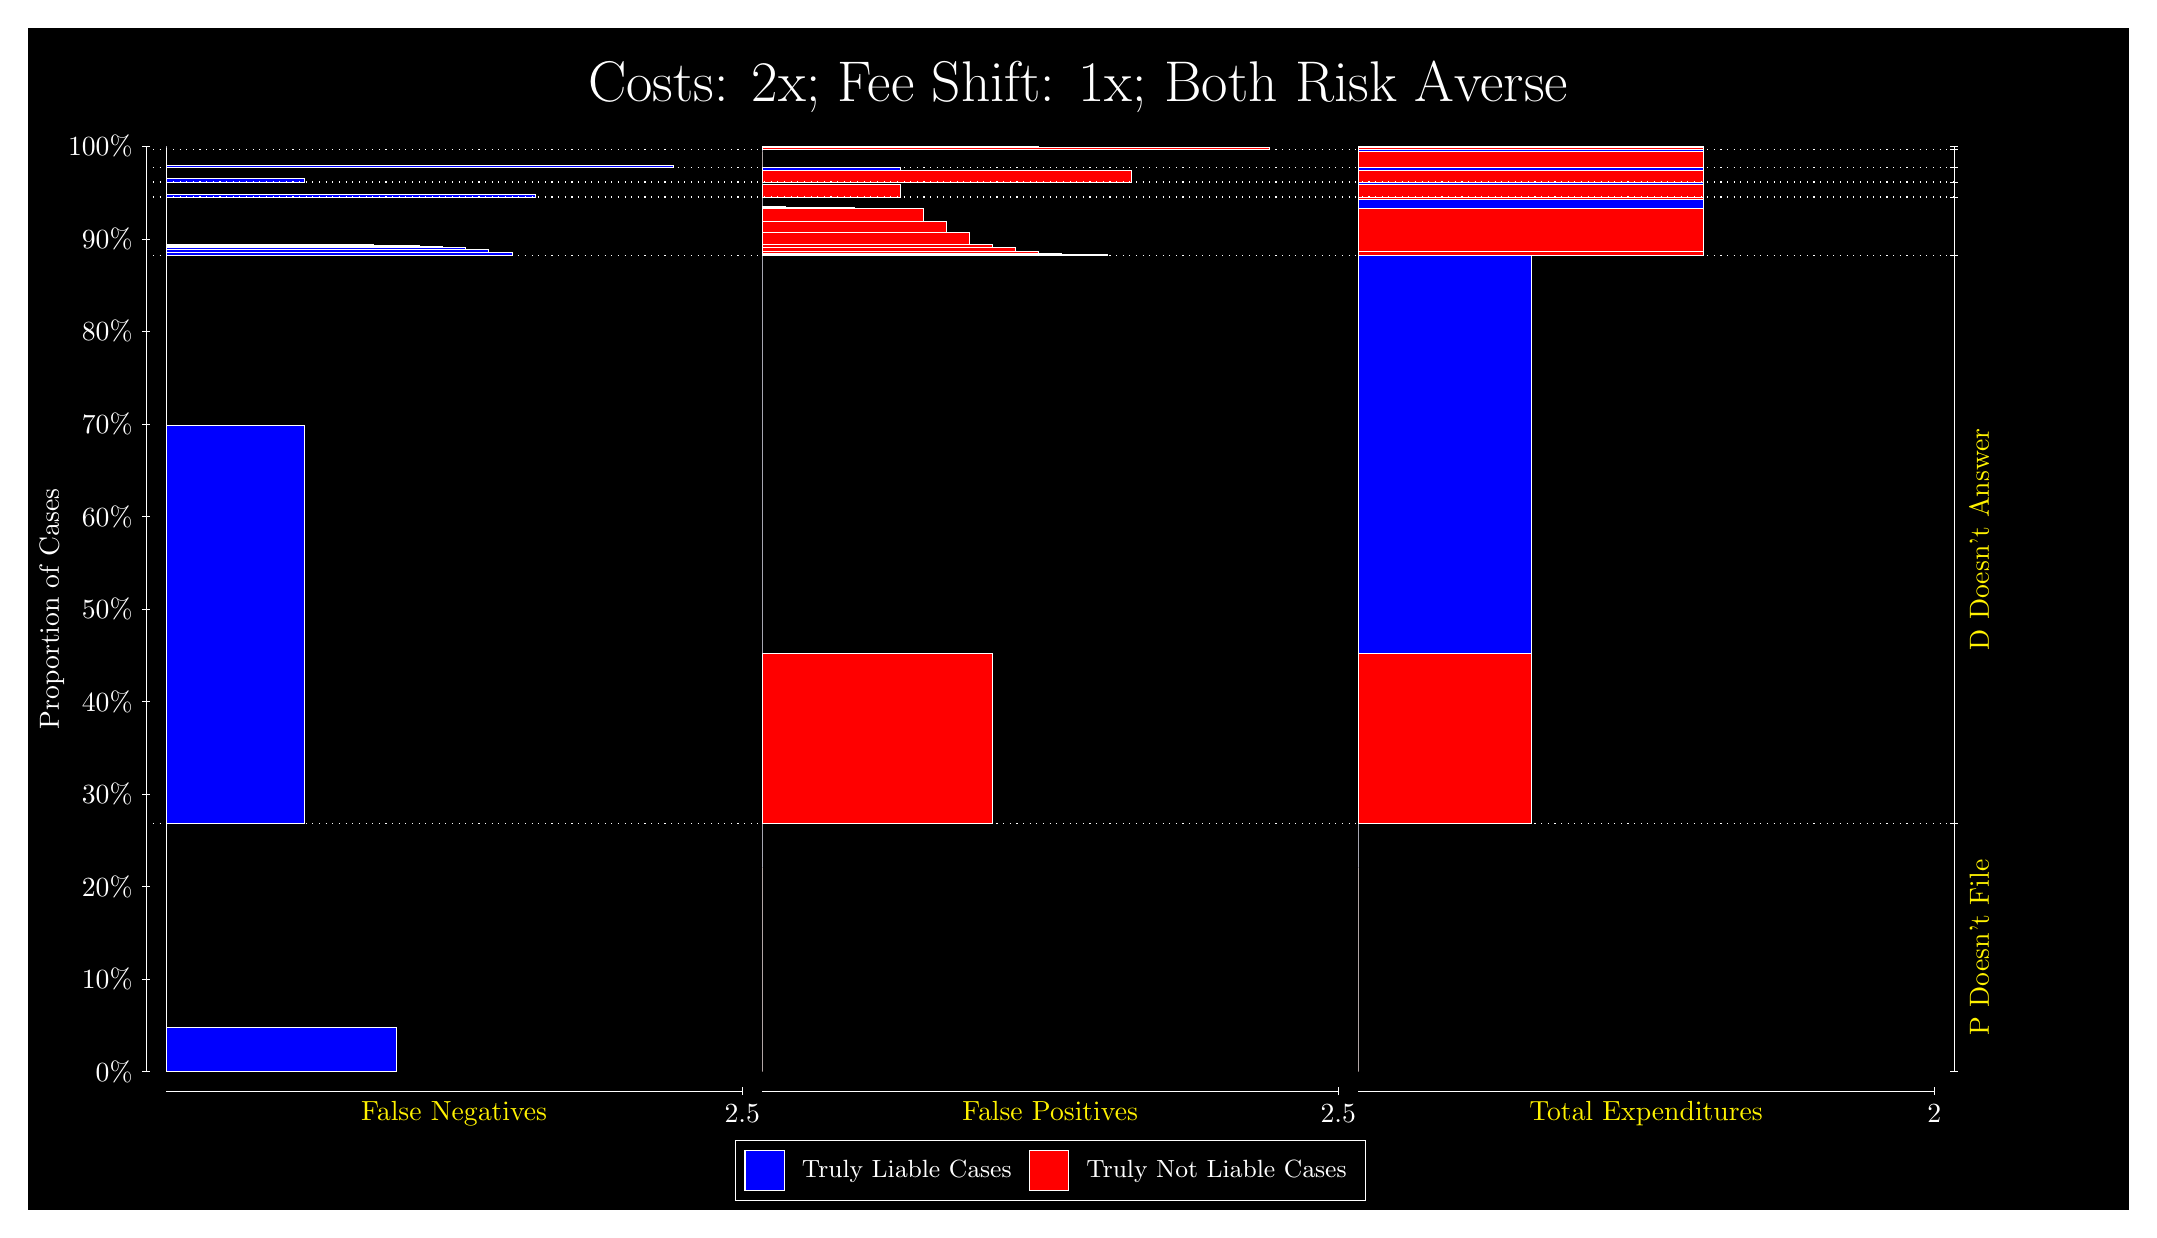
\begin{tikzpicture}
\draw[fill=black] (0,0) rectangle (26.667,15);
\draw[text=white] (0,13.5) rectangle (26.667,15) node[midway] {\huge Costs: 2x; Fee Shift: 1x; Both Risk Averse};
\draw[white, very thin] (1.5,1.75) -- (1.5,13.5);
\node[rotate=90, text=white, anchor=center] at (0.3, 7.625) {Proportion of Cases};
\draw[white, very thin] (1.45,1.75) -- (1.55,1.75);
\node[text=white, anchor=east] at (1.45, 1.75) {0\%};
\draw[white, very thin] (1.45,2.925) -- (1.55,2.925);
\node[text=white, anchor=east] at (1.45, 2.925) {10\%};
\draw[white, very thin] (1.45,4.1) -- (1.55,4.1);
\node[text=white, anchor=east] at (1.45, 4.1) {20\%};
\draw[white, very thin] (1.45,5.275) -- (1.55,5.275);
\node[text=white, anchor=east] at (1.45, 5.275) {30\%};
\draw[white, very thin] (1.45,6.45) -- (1.55,6.45);
\node[text=white, anchor=east] at (1.45, 6.45) {40\%};
\draw[white, very thin] (1.45,7.625) -- (1.55,7.625);
\node[text=white, anchor=east] at (1.45, 7.625) {50\%};
\draw[white, very thin] (1.45,8.8) -- (1.55,8.8);
\node[text=white, anchor=east] at (1.45, 8.8) {60\%};
\draw[white, very thin] (1.45,9.975) -- (1.55,9.975);
\node[text=white, anchor=east] at (1.45, 9.975) {70\%};
\draw[white, very thin] (1.45,11.15) -- (1.55,11.15);
\node[text=white, anchor=east] at (1.45, 11.15) {80\%};
\draw[white, very thin] (1.45,12.325) -- (1.55,12.325);
\node[text=white, anchor=east] at (1.45, 12.325) {90\%};
\draw[white, very thin] (1.45,13.5) -- (1.55,13.5);
\node[text=white, anchor=east] at (1.45, 13.5) {100\%};

\draw[white, very thin] (24.457,1.75) -- (24.457,13.5);
\draw[white, very thin] (24.407,1.75) -- (24.507,1.75);
\node[anchor=west] at (24.407, 1.75) {};
\draw[white, very thin] (24.407,4.9011) -- (24.507,4.9011);
\node[anchor=west] at (24.407, 4.9011) {};
\draw[white, very thin] (24.407,12.117) -- (24.507,12.117);
\node[anchor=west] at (24.407, 12.117) {};
\draw[white, very thin] (24.407,12.857) -- (24.507,12.857);
\node[anchor=west] at (24.407, 12.857) {};
\draw[white, very thin] (24.407,13.047) -- (24.507,13.047);
\node[anchor=west] at (24.407, 13.047) {};
\draw[white, very thin] (24.407,13.236) -- (24.507,13.236);
\node[anchor=west] at (24.407, 13.236) {};
\draw[white, very thin] (24.407,13.46) -- (24.507,13.46);
\node[anchor=west] at (24.407, 13.46) {};
\draw[white, very thin] (24.407,13.5) -- (24.507,13.5);
\node[anchor=west] at (24.407, 13.5) {};

\draw[white, very thin, fill=blue] (1.75,1.75) rectangle (4.6775,2.3114);
\draw[white, very thin, fill=red] (1.75,2.3114) rectangle (1.75,4.9011);
\draw[white, very thin, fill=blue] (1.75,4.9011) rectangle (3.5065,9.9599);
\draw[white, very thin, fill=red] (1.75,9.9599) rectangle (1.75,12.117);
\draw[white, very thin, fill=blue] (1.75,12.117) rectangle (6.1413,12.16);
\draw[white, very thin, fill=blue] (1.75,12.16) rectangle (5.8486,12.191);
\draw[white, very thin, fill=blue] (1.75,12.191) rectangle (5.5558,12.221);
\draw[white, very thin, fill=blue] (1.75,12.221) rectangle (5.2631,12.231);
\draw[white, very thin, fill=blue] (1.75,12.231) rectangle (4.9703,12.242);
\draw[white, very thin, fill=blue] (1.75,12.242) rectangle (4.6775,12.248);
\draw[white, very thin, fill=blue] (1.75,12.248) rectangle (4.3848,12.252);
\draw[white, very thin, fill=blue] (1.75,12.252) rectangle (4.092,12.254);
\draw[white, very thin, fill=blue] (1.75,12.254) rectangle (3.7993,12.256);
\draw[white, very thin, fill=red] (1.75,12.256) rectangle (1.75,12.857);
\draw[white, very thin, fill=blue] (1.75,12.857) rectangle (6.4341,12.885);
\draw[white, very thin, fill=red] (1.75,12.885) rectangle (1.75,13.047);
\draw[white, very thin, fill=blue] (1.75,13.047) rectangle (3.5065,13.093);
\draw[white, very thin, fill=red] (1.75,13.093) rectangle (1.75,13.236);
\draw[white, very thin, fill=blue] (1.75,13.236) rectangle (8.1906,13.261);
\draw[white, very thin, fill=red] (1.75,13.261) rectangle (1.75,13.46);
\draw[white, very thin, fill=red] (1.75,13.46) rectangle (1.75,13.484);
\draw[white, very thin, fill=blue] (1.75,13.484) rectangle (1.75,13.5);
\draw[white, very thin, fill=red] (9.3189,1.75) rectangle (9.3189,4.3397);
\draw[white, very thin, fill=blue] (9.3189,4.3397) rectangle (9.3189,4.9011);
\draw[white, very thin, fill=red] (9.3189,4.9011) rectangle (12.246,7.0579);
\draw[white, very thin, fill=blue] (9.3189,7.0579) rectangle (9.3189,12.117);
\draw[white, very thin, fill=red] (9.3189,12.117) rectangle (13.71,12.123);
\draw[white, very thin, fill=red] (9.3189,12.123) rectangle (13.417,12.13);
\draw[white, very thin, fill=red] (9.3189,12.13) rectangle (13.125,12.144);
\draw[white, very thin, fill=red] (9.3189,12.144) rectangle (12.832,12.17);
\draw[white, very thin, fill=red] (9.3189,12.17) rectangle (12.539,12.215);
\draw[white, very thin, fill=red] (9.3189,12.215) rectangle (12.246,12.252);
\draw[white, very thin, fill=red] (9.3189,12.252) rectangle (11.954,12.41);
\draw[white, very thin, fill=red] (9.3189,12.41) rectangle (11.661,12.544);
\draw[white, very thin, fill=red] (9.3189,12.544) rectangle (11.368,12.717);
\draw[white, very thin, fill=blue] (9.3189,12.717) rectangle (10.783,12.719);
\draw[white, very thin, fill=blue] (9.3189,12.719) rectangle (10.49,12.721);
\draw[white, very thin, fill=blue] (9.3189,12.721) rectangle (10.197,12.725);
\draw[white, very thin, fill=blue] (9.3189,12.725) rectangle (9.9044,12.731);
\draw[white, very thin, fill=blue] (9.3189,12.731) rectangle (9.6116,12.743);
\draw[white, very thin, fill=blue] (9.3189,12.743) rectangle (9.3189,12.857);
\draw[white, very thin, fill=red] (9.3189,12.857) rectangle (11.075,13.019);
\draw[white, very thin, fill=blue] (9.3189,13.019) rectangle (9.3189,13.047);
\draw[white, very thin, fill=red] (9.3189,13.047) rectangle (14.003,13.19);
\draw[white, very thin, fill=blue] (9.3189,13.19) rectangle (11.075,13.236);
\draw[white, very thin, fill=red] (9.3189,13.236) rectangle (9.3189,13.435);
\draw[white, very thin, fill=blue] (9.3189,13.435) rectangle (9.3189,13.46);
\draw[white, very thin, fill=red] (9.3189,13.46) rectangle (15.759,13.484);
\draw[white, very thin, fill=blue] (9.3189,13.484) rectangle (12.832,13.5);
\draw[white, very thin, fill=red] (16.888,1.75) rectangle (16.888,4.3397);
\draw[white, very thin, fill=blue] (16.888,4.3397) rectangle (16.888,4.9011);
\draw[white, very thin, fill=red] (16.888,4.9011) rectangle (19.083,7.0579);
\draw[white, very thin, fill=blue] (16.888,7.0579) rectangle (19.083,12.117);
\draw[white, very thin, fill=red] (16.888,12.117) rectangle (21.279,12.161);
\draw[white, very thin, fill=blue] (16.888,12.161) rectangle (21.279,12.173);
\draw[white, very thin, fill=red] (16.888,12.173) rectangle (21.279,12.708);
\draw[white, very thin, fill=blue] (16.888,12.708) rectangle (21.279,12.83);
\draw[white, very thin, fill=red] (16.888,12.83) rectangle (21.279,12.851);
\draw[white, very thin, fill=blue] (16.888,12.851) rectangle (21.279,12.857);
\draw[white, very thin, fill=red] (16.888,12.857) rectangle (21.279,13.019);
\draw[white, very thin, fill=blue] (16.888,13.019) rectangle (21.279,13.047);
\draw[white, very thin, fill=red] (16.888,13.047) rectangle (21.279,13.19);
\draw[white, very thin, fill=blue] (16.888,13.19) rectangle (21.279,13.236);
\draw[white, very thin, fill=red] (16.888,13.236) rectangle (21.279,13.435);
\draw[white, very thin, fill=blue] (16.888,13.435) rectangle (21.279,13.46);
\draw[white, very thin, fill=red] (16.888,13.46) rectangle (21.279,13.484);
\draw[white, very thin, fill=blue] (16.888,13.484) rectangle (21.279,13.5);
\draw[white, dotted] (1.5,4.9011) -- (24.457,4.9011);
\draw[white, dotted] (1.5,12.117) -- (24.457,12.117);
\draw[white, dotted] (1.5,12.857) -- (24.457,12.857);
\draw[white, dotted] (1.5,13.047) -- (24.457,13.047);
\draw[white, dotted] (1.5,13.236) -- (24.457,13.236);
\draw[white, dotted] (1.5,13.46) -- (24.457,13.46);
\draw[white, very thin] (1.75,1.5) -- (9.0689,1.5);
\node[text=yellow, anchor=north] at (5.4094, 1.5) {False Negatives};
\draw[white, very thin] (9.0689,1.45) -- (9.0689,1.55);
\node[text=white, anchor=north] at (9.0689, 1.45) {2.5};

\draw[white, very thin] (9.3189,1.5) -- (16.638,1.5);
\node[text=yellow, anchor=north] at (12.978, 1.5) {False Positives};
\draw[white, very thin] (16.638,1.45) -- (16.638,1.55);
\node[text=white, anchor=north] at (16.638, 1.45) {2.5};

\draw[white, very thin] (16.888,1.5) -- (24.207,1.5);
\node[text=yellow, anchor=north] at (20.547, 1.5) {Total Expenditures};
\draw[white, very thin] (24.207,1.45) -- (24.207,1.55);
\node[text=white, anchor=north] at (24.207, 1.45) {2};

\node[text=yellow, centered, rotate=90] at (24.777, 3.3255) {P Doesn't File};
\node[text=yellow, centered, rotate=90] at (24.777, 8.5089) {D Doesn't Answer};






\draw (12.978300999999998,1.5) node[draw=none] (baseCoordinate) {};
\begin{scope}[align=center]
        \matrix[scale=0.5, draw=white, below=0.5cm of baseCoordinate, nodes={draw}, column sep=0.1cm]{
            \node[rectangle, draw, minimum width=0.5cm, minimum height=0.5cm, fill=blue] {}; &
            \node[draw=none, font=\small, text=white] (B) {Truly Liable Cases}; &
            \node[rectangle, draw, minimum width=0.5cm, minimum height=0.5cm, fill=red] {}; &
            \node[draw=none, font=\small, text=white] (B) {Truly Not Liable Cases}; \\
            };
\end{scope}

\end{tikzpicture}
\end{document}